\section{Vandermondeova determinanta}

Za $n$ zadanih točaka ($x_k$, $y_k$) gdje je $y_k := f(x_k)$, $k$ predstavlja indeks točke ($k = 0, 1, \dots, n$), ako ni jedne dvije točke nemaju istu $x$ vrijednost postoji jedinstveni \textbf{interpolacijski polinom} najviše stupnja $n$:
\begin{equation}
    p_n(x)\coloneq \sum_{i=0}^na_ix^i= a_0 + a_1x + \dots a_nx^n
\end{equation}

Sustavi dobiveni uporabom vandermondeove determinante su nestabilni te se zbog toga najčešće koristi baza polinoma koja daje stabilnije rezultate.

\begin{example}[uporaba vandermondeove determinante]
    Zadane su sljedeće točke, odredi interpolacijski polinom uporabom vandermondeove determinante:

    \center
    \begin{tabular}{r|c|c|c}
        $x$&0&2&4\\
        \hline
        $y$&3&4&2
    \end{tabular}
\end{example}

\begin{multicols}{2}

Zadane su 3 točke pa očekujemo polinom maksimalno drugog stupnja:

$$
    p_2(x) = a_0 + a_1x + a_2x^2
$$

Uvrštavanjem točaka dobivamo:

\begin{gather*}
p_2(0) = a_0\cdot 1 + a_1\cdot 0 + a_2\cdot 0^2 = 3\\
p_2(2) = a_0\cdot 1 + a_1\cdot 2 + a_2\cdot 2^2 = 4\\
p_2(4) = a_0\cdot 1 + a_1\cdot 4 + a_2\cdot 4^2 = 2
\end{gather*}

\newcolumn

Što predstavljeno kao matrična jednadžba izgleda kao:

\begin{gather*}
\begin{bmatrix}
1 & 0 & 0 \\
1 & 2 & 4 \\
1 & 4 & 16
\end{bmatrix}
\cdot
\begin{bmatrix}
a_0 \\ a_1 \\ a_2
\end{bmatrix}
=
\begin{bmatrix}
3 \\ 4 \\ 2
\end{bmatrix} \\\\
A\cdot X = B \\
X = A^{-1} \cdot B
\end{gather*}

\end{multicols}

Zatim računamo \textbf{vandermondeovu determinantu}:

$$
D_n =
det(A) =
\begin{vmatrix}
1 & 0 & 0 \\
1 & 2 & 4 \\
1 & 4 & 16
\end{vmatrix}
= 1 \cdot
\begin{vmatrix}
2 & 4 \\
4 & 16
\end{vmatrix}
= 32 - 16 = 16 \neq 0
$$

\begin{multicols}{2}

Kako bismo odredili $A^{-1}$ trebamo provjeriti da je $det(A)\neq0$, u suprotnom inverzna matrica ne postoji. U ovom primjeru, inverzna matrica je:

\begin{gather*}
A^{-1} =
\begin{bmatrix}
1 & 0 & 0\\
-{\frac{3}{4}} & 1 & -{\frac{1}{4}}\\
{\frac{1}{8}} & -{\frac{1}{4}} & {\frac{1}{8}}
\end{bmatrix}\\
X = A^{-1}\cdot B =
\begin{bmatrix}
1 & 0 & 0\\
-\frac{3}{4} & 1 & -\frac{1}{4}\\
\frac{1}{8} & -\frac{1}{4} & \frac{1}{8}
\end{bmatrix}
\cdot
\begin{bmatrix}
3 \\ 4 \\ 2
\end{bmatrix}
=
\begin{bmatrix}
3 \\ \frac{5}{4} \\ -\frac{3}{8}
\end{bmatrix}
\end{gather*}

Rješavanjem sustava dobivamo $a_0=3$, $a_1=\frac{5}{4}$,\break$a_2=-\frac{3}{8}$,
kao i interpolaciju funkcije:
$$
p_2(x) = 3 + \frac{5}{4}x - \frac{3}{8}x^2
$$

\newcolumn

\vspace*{0pt}

\begin{tikzpicture}
    \begin{axis}[
        xmin=-1,xmax=5,
        ymin=-1,ymax=6
    ]
        \addplot[plotlinefound] expression[samples=100]{3 + 5/4*x - 3/8*x^2} node[pos=0.8,anchor=south west]{$y=\sin{2x}+\frac{1}{2}$};
        \addplot[plotinterpolated] coordinates {(0,3)};
        \addplot[plotinterpolated] coordinates {(2,4)};
        \addplot[plotinterpolated] coordinates {(4,2)};
    \end{axis}
\end{tikzpicture}

\end{multicols}

\pagebreak

\subsection{Rješavanje sustava jednadžbi u Pythonu}

\begin{example}
    Odredite interpolacijski polinom uporabom vandermondeove determinante u
    Pythonu za točke iz prethodnog primjera.
\end{example}

\begin{multicols}{2}
    \section{Vandermondeova determinanta}

Za $n$ zadanih točaka ($x_k$, $y_k$) gdje je $y_k := f(x_k)$, $k$ predstavlja indeks točke ($k = 0, 1, \dots, n$), ako ni jedne dvije točke nemaju istu $x$ vrijednost postoji jedinstveni \textbf{interpolacijski polinom} najviše stupnja $n$:
\begin{equation}
    p_n(x)\coloneq \sum_{i=0}^na_ix^i= a_0 + a_1x + \dots a_nx^n
\end{equation}

Sustavi dobiveni uporabom vandermondeove determinante su nestabilni te se zbog toga najčešće koristi baza polinoma koja daje stabilnije rezultate.

\begin{example}[uporaba vandermondeove determinante]
    Zadane su sljedeće točke, odredi interpolacijski polinom uporabom vandermondeove determinante:

    \center
    \begin{tabular}{r|c|c|c}
        $x$&0&2&4\\
        \hline
        $y$&3&4&2
    \end{tabular}
\end{example}

\begin{multicols}{2}

Zadane su 3 točke pa očekujemo polinom maksimalno drugog stupnja:

$$
    p_2(x) = a_0 + a_1x + a_2x^2
$$

Uvrštavanjem točaka dobivamo:

\begin{gather*}
p_2(0) = a_0\cdot 1 + a_1\cdot 0 + a_2\cdot 0^2 = 3\\
p_2(2) = a_0\cdot 1 + a_1\cdot 2 + a_2\cdot 2^2 = 4\\
p_2(4) = a_0\cdot 1 + a_1\cdot 4 + a_2\cdot 4^2 = 2
\end{gather*}

\newcolumn

Što predstavljeno kao matrična jednadžba izgleda kao:

\begin{gather*}
\begin{bmatrix}
1 & 0 & 0 \\
1 & 2 & 4 \\
1 & 4 & 16
\end{bmatrix}
\cdot
\begin{bmatrix}
a_0 \\ a_1 \\ a_2
\end{bmatrix}
=
\begin{bmatrix}
3 \\ 4 \\ 2
\end{bmatrix} \\\\
A\cdot X = B \\
X = A^{-1} \cdot B
\end{gather*}

\end{multicols}

Zatim računamo \textbf{vandermondeovu determinantu}:

$$
D_n =
det(A) =
\begin{vmatrix}
1 & 0 & 0 \\
1 & 2 & 4 \\
1 & 4 & 16
\end{vmatrix}
= 1 \cdot
\begin{vmatrix}
2 & 4 \\
4 & 16
\end{vmatrix}
= 32 - 16 = 16 \neq 0
$$

\begin{multicols}{2}

Kako bismo odredili $A^{-1}$ trebamo provjeriti da je $det(A)\neq0$, u suprotnom inverzna matrica ne postoji. U ovom primjeru, inverzna matrica je:

\begin{gather*}
A^{-1} =
\begin{bmatrix}
1 & 0 & 0\\
-{\frac{3}{4}} & 1 & -{\frac{1}{4}}\\
{\frac{1}{8}} & -{\frac{1}{4}} & {\frac{1}{8}}
\end{bmatrix}\\
X = A^{-1}\cdot B =
\begin{bmatrix}
1 & 0 & 0\\
-\frac{3}{4} & 1 & -\frac{1}{4}\\
\frac{1}{8} & -\frac{1}{4} & \frac{1}{8}
\end{bmatrix}
\cdot
\begin{bmatrix}
3 \\ 4 \\ 2
\end{bmatrix}
=
\begin{bmatrix}
3 \\ \frac{5}{4} \\ -\frac{3}{8}
\end{bmatrix}
\end{gather*}

Rješavanjem sustava dobivamo $a_0=3$, $a_1=\frac{5}{4}$,\break$a_2=-\frac{3}{8}$,
kao i interpolaciju funkcije:
$$
p_2(x) = 3 + \frac{5x}{4} + -\frac{3x^2}{8}
$$

\newcolumn

\vspace*{0pt}

\begin{tikzpicture}
    \begin{axis}[
        xmin=-1,xmax=5,
        ymin=-1,ymax=6
    ]
        \addplot[plotlinefound] expression[samples=100]{3 + 5/4*x - 3/8*x^2} node[pos=0.8,anchor=south west]{$y=\sin{2x}+\frac{1}{2}$};
        \addplot[plotinterpolated] coordinates {(0,3)};
        \addplot[plotinterpolated] coordinates {(2,4)};
        \addplot[plotinterpolated] coordinates {(4,2)};
    \end{axis}
\end{tikzpicture}

\end{multicols}


    \columnbreak

    \textbf{Ispis}

    \begin{verbatim}
    Rješenje sustava: [ 3.     1.25  -0.375]
    p(0) = 3.0
    p(2) = 4.0
    p(4) = 2.0
    \end{verbatim}

    \textbf{Rezultat prikaza}

    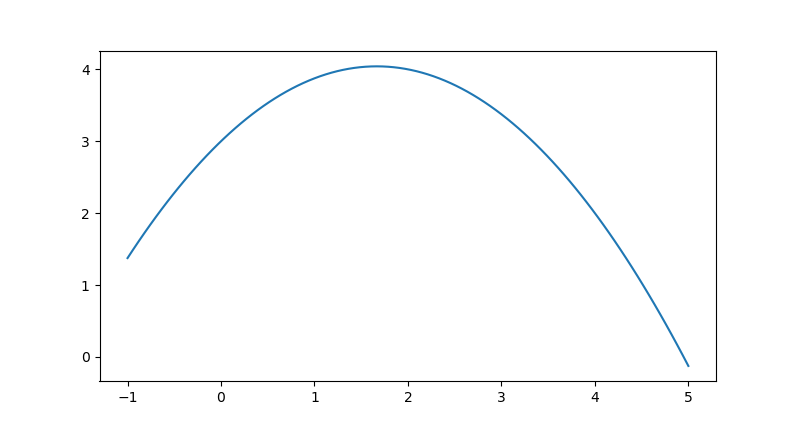
\includegraphics[width=\linewidth]{fig/vandermond.png}

\end{multicols}
